\documentclass[tikz,border=8pt]{standalone}
% Shared look for every TikZ diagram. Load with \input{../../tools/tikz-style.tex}
\usepackage[T1]{fontenc}
\usepackage{lmodern}
\renewcommand{\sfdefault}{lmr}  % diagrams use the same serif as the text
\usetikzlibrary{arrows.meta, positioning, shapes.geometric, calc, fit, backgrounds}
\definecolor{cblue}{HTML}{4C78A8}
\definecolor{corange}{HTML}{F58518}
\definecolor{cgreen}{HTML}{54A24B}
\definecolor{cred}{HTML}{E45756}
\definecolor{cpurple}{HTML}{B279A2}
\definecolor{cgrey}{HTML}{6B6B6B}
\tikzset{
  every picture/.style={font=\sffamily, line width=1.2pt},
  box/.style={draw=#1, fill=#1!12, rounded corners=4pt, align=center, inner sep=7pt, minimum height=1.1cm},
  box/.default=cgrey,
  arrow/.style={-{Stealth[length=3mm]}, draw=cgrey, line width=1.4pt},
  title/.style={font=\sffamily\bfseries\Large},
  note/.style={font=\sffamily\small, text=cgrey, align=center},
}
\AtBeginDocument{\hyphenpenalty=10000 \exhyphenpenalty=10000}

% Room 5 m x 4 m, robot at pose (2, 2, 0). Four beams at 0, 90, 180, 270 degrees. Expected ranges 3, 2, 2, 2 m.
% A person stands 1 m ahead, so the forward beam reads 1.00 m instead of 3 m. Readings: 1.00, 1.97, 2.04, 1.99.
\begin{document}
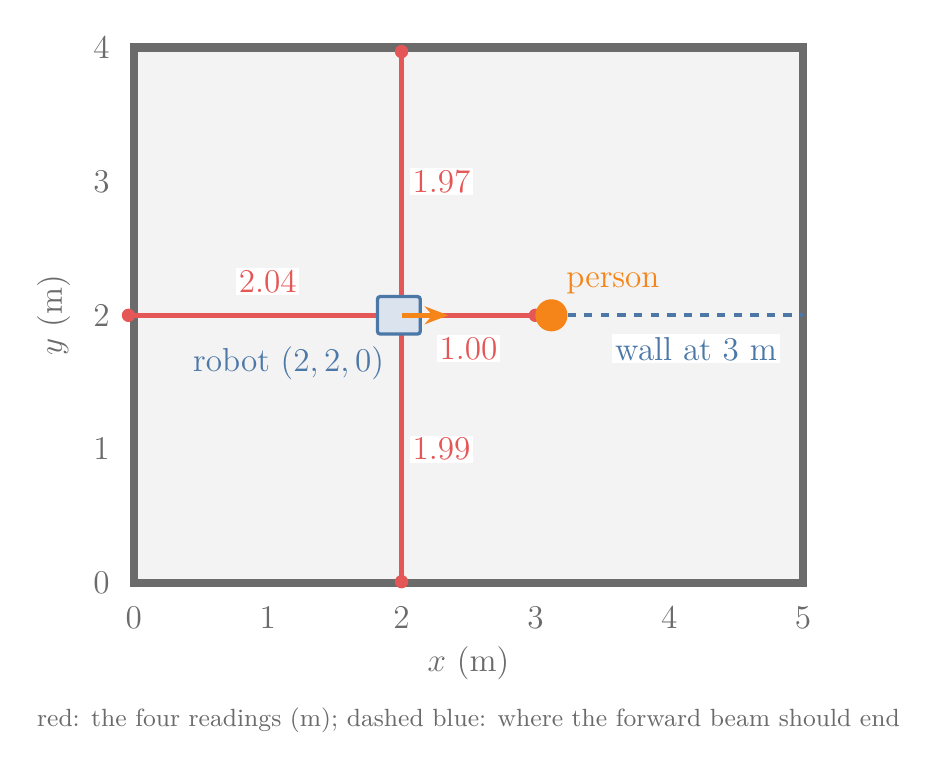
\begin{tikzpicture}[scale=1.7, every node/.append style={font=\large}]
  \fill[cgrey!8] (0,0) rectangle (5,4);
  \draw[cgrey, line width=3pt] (0,0) rectangle (5,4);
  \foreach \x in {0,1,...,5} \node[below, cgrey] at (\x,-0.1) {\x};
  \foreach \y in {0,1,...,4} \node[left, cgrey] at (-0.1,\y) {\y};
  \node[cgrey] at (2.5,-0.6) {$x$ (m)};
  \node[cgrey, rotate=90] at (-0.6,2) {$y$ (m)};
  % expected beams (dashed, to the walls)
  \draw[cblue, dashed, line width=1.4pt] (2,2) -- (5,2);
  % actual beams (solid red, to where the reading ends)
  \draw[cred, line width=2pt] (2,2) -- (3,2);
  \draw[cred, line width=2pt] (2,2) -- (2,3.97);
  \draw[cred, line width=2pt] (2,2) -- (-0.04+0.0,2) ;
  \draw[cred, line width=2pt] (2,2) -- (2,0.01);
  \foreach \p in {(3,2),(2,3.97),(-0.04,2),(2,0.01)} \fill[cred] \p circle (0.05);
  % person
  \fill[corange] (3.12,2) circle (0.12);
  \node[corange, above right] at (3.15,2.08) {person};
  % robot
  \draw[cblue, fill=cblue!20, rounded corners=1pt] (1.82,1.86) rectangle (2.14,2.14);
  \draw[-{Stealth[length=3mm]}, corange, line width=2pt] (2,2) -- (2.35,2);
  % labels
  \node[cred, fill=white, inner sep=1pt] at (2.5,1.75) {$1.00$};
  \node[cblue, fill=white, inner sep=1pt] at (4.2,1.75) {wall at $3$ m};
  \node[cred, fill=white, inner sep=1pt, right] at (2.05,3.0) {$1.97$};
  \node[cred, fill=white, inner sep=1pt] at (1.0,2.25) {$2.04$};
  \node[cred, fill=white, inner sep=1pt, right] at (2.05,1.0) {$1.99$};
  \node[cblue, below left] at (1.95,1.85) {robot $(2, 2, 0)$};
  \node[note, anchor=north] at (2.5,-0.85) {red: the four readings (m); dashed blue: where the forward beam should end};
\end{tikzpicture}
\end{document}
